\documentclass[12pt,a4paper]{article}
\usepackage{times}
\usepackage[utf8]{inputenc}
\usepackage[czech]{babel}
\usepackage[left=1.5cm, top=1.5cm, text={18cm, 26cm}]{geometry}
\usepackage{graphicx} % figures (\includegraphics...)
\usepackage{float} % figures positioning ([H])
\usepackage[unicode]{hyperref} % \ref{...}
\urlstyle{same} % \ref{...}
\renewcommand{\figurename}{Obrázek}

\usepackage{amsfonts} % natural numbers -> \mathbb{N}

\usepackage{fancyhdr}
\pagestyle{fancy}
\fancyhf{}
\renewcommand{\headrulewidth}{0pt}
\lfoot{PRL Projekt}
\rfoot{Michal Sova}
\cfoot{\thepage}

%\title{Projekt do předmětu PRL - Odd-Even Merge Sort}
%\author{Michal Sova (xsovam00@stud.fit.vutbr.cz)}

\begin{document}
%\maketitle

\section{Odd-Even Merge Sort}
\label{sec:odd_even_merge_sort}
Základní jednotkou algoritmu Odd-Even Merge Sort je komparátor (Obr. \ref{fig:net1x1}). 
Ten obdrží dva vstupy, a vrací dva výstupy. Jedinou operací komarátoru je porovnat tyto dva vstupy a na výstup dát seřazenou posloupnost těchto dvou vstupů.
Použitím těchto komarátorů lze vytvořit síť, která má na vstupu dvě seřazené posloupnosti $A = \{a_1, a_2, ..., a_n\}$ a $B = \{b_1, b_2, ..., b_n\}$ a na výstupu má seřazenou posloupnost $C = \{c_1, c_2, ..., c_{2n}\}$, kde $n$ je mocninou 2. 
Pro seřazení dvou již seřazených posloupností $A = \{a_1, a_2\}$ a $B = \{b_1, b_2\}$ lze použít síť na Obr. \ref{fig:net2x2}. 
Tímto způsobem lze sestavit kaskádu sítí pro seřazení $n = 2^m$ čísel, kde $m \in \mathbb{N}$ čísel. 
Na Obr. \ref{fig:oems} lze vidět případ Odd-Even Merge Sort pro 8 čísel.
\begin{figure}[H]
\centering
    \begin{minipage}{.45\textwidth}
        \centering
        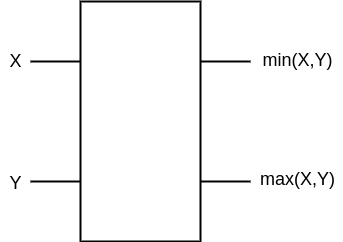
\includegraphics[width=.9\textwidth]{img/comparator.png}
        \caption{Komparátor}
        \label{fig:net1x1}
    \end{minipage}
    \hfill
    \begin{minipage}{.5\textwidth}
        \centering
        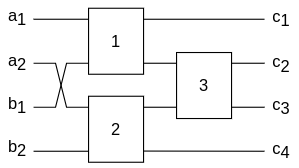
\includegraphics[width=.9\textwidth]{img/net2x2.png}
        \caption{Síť 2$\times$2}
        \label{fig:net2x2}
    \end{minipage}
\end{figure}

\subsection*{Časová složitost}
\label{sub:casova_slozitost}
Uvažujme, že komparátor načítá svůj vstup, porovnává ho a generuje výstup v jednu časovou jednotku. 
Pak pro $n = 2^m, m > 0, m \in \mathbb{N}$ čísel lze zapsat:

\begin{equation}
    t(2) = 1
\end{equation}
\begin{equation}
    t(2^m) = t(2^{m-1}) + m
\end{equation}
Kde obecně $t(x)$ udává čas potřebný pro uspořádání posloupnosti o velikosti $x$.
Z toho lze odvodit
\begin{equation}
    t(2^m) = \sum_{i=1}^{m} i
\end{equation}
\begin{equation}
    t(n) = \sum_{i=1}^{\log n} i \rightarrow t(n) = \mathcal{O}(\log^2 n)
    \label{eq:cas}
\end{equation}
Výsledná časová složitost algoritmu je tedy $\mathcal{O}(\log^2 n)$.

\subsection*{Počet procesorů}
\label{sub:pocet_procesoru}

Řadíme posloupnost obecně o délce $n = 2^m, m > 0, m \in \mathbb{N}$. Pak potřebujeme dvě sítě k seřazení dvou posloupností o velikosti $2^{m-1}$ a jednu síť ke spojení těchto dvou seřazených posloupností.
Z tohoto můžeme odvodit:

\begin{equation}
    p(2) = 1
\end{equation}
\begin{equation}
    p(2^m) = 2 * p(2^{m-1}) + 2^{m-1} * (m - 1) + 1
\end{equation}
kde obecně $p(x)$ udává počet procesorů potřebných pro seřazení posloupnosti o velikosti $x$.
Tento vztah lze opět uravit 
\begin{equation}
    p(n) = \sum_{i=1}^{m} 2^{m-i} * (2^{i-1} * (i-1) + 1)
\end{equation}
\begin{equation}
    p(n) = \sum_{i=1}^{\log n} 2^{(\log n)-i} * (2^{i-1} * (i-1) + 1) \rightarrow p(n) = \mathcal{O}(n \log^2 n)
    \label{eq:prostor}
\end{equation}
Prostorová složitost je tedy $\mathcal{O}(n \log^2 n)$.

\subsection*{Celková cena}
\label{sub:celkova_cena}
Celkovou cenu $c(n)$ lze odvodit:
\begin{equation}
    c(n) = p(n) \times t(n)
\end{equation}
\begin{equation}
    c(n) = \mathcal{O}(n\log^2 n) \times \mathcal{O}(\log^2 n)
\end{equation}
\begin{equation}    
    c(n) = \mathcal{O}(n \log^4 n)
    \label{eq:cena}
\end{equation}

\section{Implementace}
\label{sec:implementace}
K implementaci Odd-Even Merge Sort pro 8 čísel je potřeba 19 procesorů. Algoritmus je implementován pomocí knihovny \texttt{OpenMPI}. Dále je vytvořena funkce simulující komparátor, funkce simulující síť 2$\times$2 a funkce sítě 4$\times$4. Argumenty funkcí pro sítě 2$\times$2 a 4$\times$4 jsou:
\begin{itemize}
     \item seřazené vstupní posloupnosti (s poloviční velikostí výstupní posloupnosti)
     \item pořadí procesoru, který volá danou funkci
     \item vektor pořadí procesorů, simulující tuto síť
 \end{itemize}
Tyto funkce vracejí spojenou seřazenou posloupnost.
Schéma algoritmu s pevným pořadím procesorů je na Obr. \ref{fig:oems}. 

Pro načtení hodnot si procesory 0-3 zavolají funkci \texttt{get\_input}, která načítá a vrací 8 bytů ze souboru \texttt{numbers}. Následně procesor 0 vypíše aktuální posloupnost a procesory 0-3 zavolají funkci \texttt{net\_1x1} simulující komparátor.
po seřazení své posloupnosti pošlou příslušným procesorům pomocí funkce \texttt{MPI\_Send}. Tyto procesory spolu s dalšími příslušnými procesory zavolají funkci \texttt{net\_2x2} simulující síť 2$\times$2. Po seřazení posloupností jsou opět tyto posloupnosti odeslány příslušným procesorům, kteří po obdržení simulují síť 4$\times$4. Plně seřazenou posloupnost si poskládá procesor 0, který ji vypíše na standatdní výstup.

\begin{figure}[H]
    \centering
    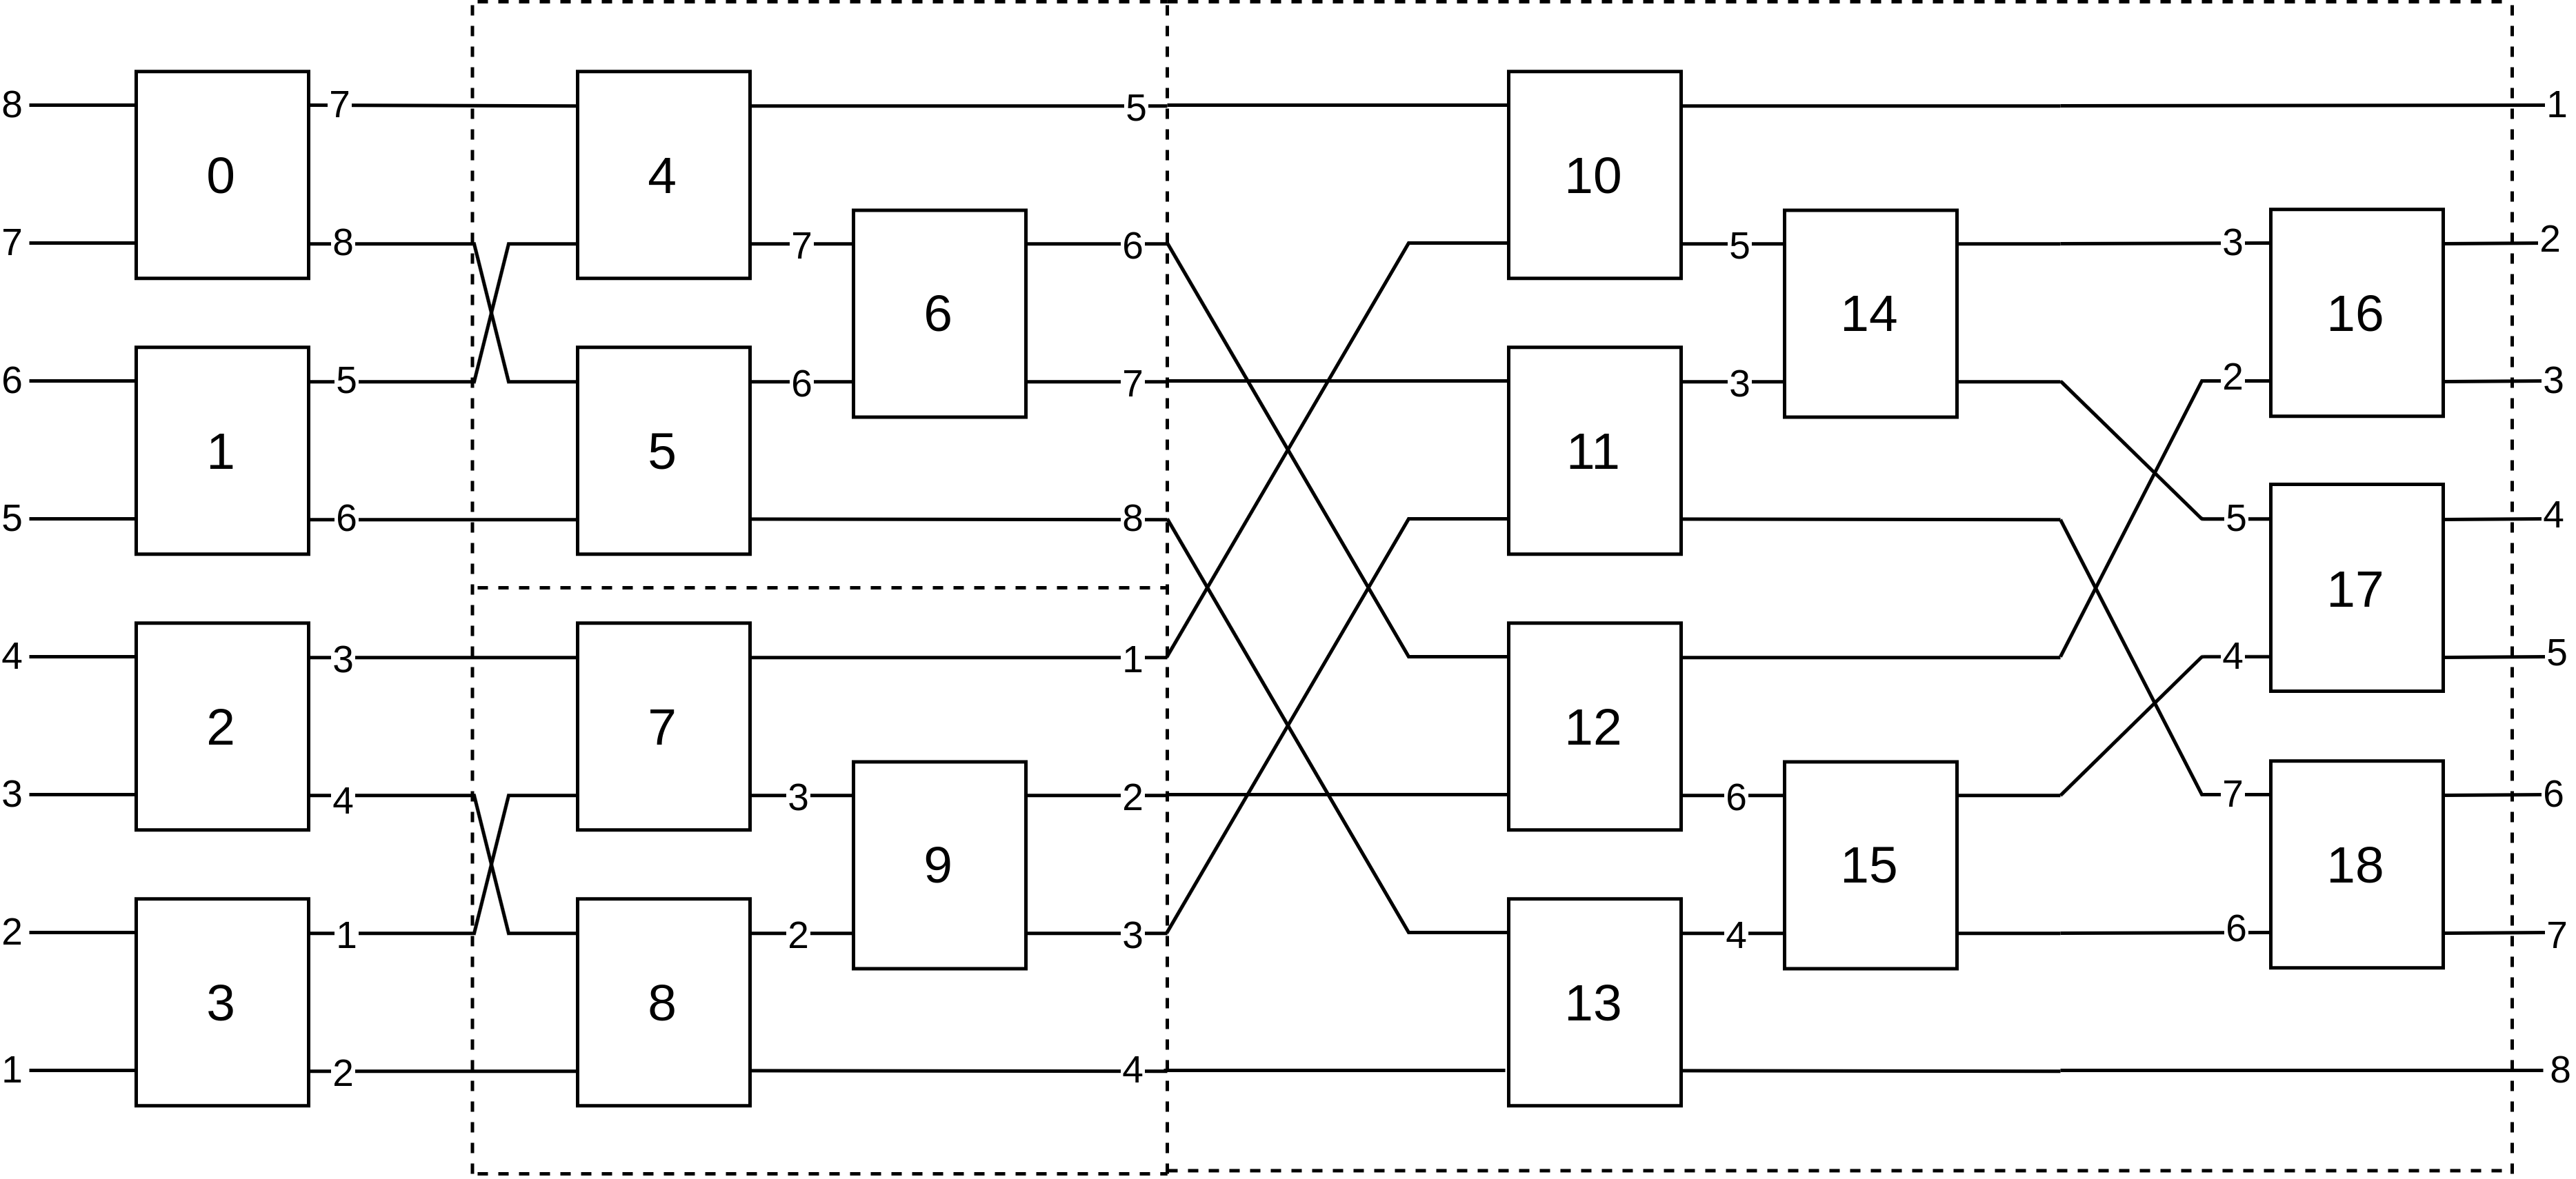
\includegraphics[width=\textwidth]{img/oems.png}
    \caption{Odd-Even Merge Sort pro 8 čísel}
    \label{fig:oems}
\end{figure}

\section{Závěr}
\label{sec:závěr}
Jak lze vidět v rovnici \ref{eq:cena} cena není optimální. Přesto má algoritmus relativně nízkou časovou složitost (rovnice \ref{eq:cas}). 

Implementovaný algoritmus je funkční a řadí dle očekávání.


\end{document}
